\documentclass[9pt,twocolumn,twoside,lineno]{pnas-new}
% Use the lineno option to display guide line numbers if required.

\templatetype{pnasresearcharticle} % Choose template 

\usepackage{natbib}

\newcommand{\tom}[2]{{\color{red}{#1}}\footnote{\textit{\color{red}{#2}}}}
\newcommand{\jacob}[2]{{\color{blue}{#1}}\footnote{\textit{\color{blue}{#2}}}}
% {pnasresearcharticle} = Template for a two-column research article
% {pnasmathematics} %= Template for a one-column mathematics article
% {pnasinvited} %= Template for a PNAS invited submission

\title{Forecasting range shifts of a dioecious plant species under climate change}

% Use letters for affiliations, numbers to show equal authorship (if applicable) and to indicate the corresponding author
\author[a,c,1]{Jacob K. Moutouama\, \textit{0000-0003-1599-1671}}
\author[b]{Aldo Compagnoni\,\textit{0000-0001-8302-7492}} 
\author[a]{Tom E.X. Miller\,\textit{0000-0003-3208-6067}}

\affil[a]{Program in Ecology and Evolutionary Biology, Department of BioSciences, Rice University, Houston, Texas, USA}
\affil[b]{Institute of Biology, Martin Luther University Halle-Wittenberg, Halle, Germany; and German Centre for Integrative Biodiversity Research (iDiv), Leipzig, Germany}
% Please give the surname of the lead author for the running footer
\leadauthor{Moutouama} 

% Please add here a significance statement to explain the relevance of your work
\significancestatement{The majority of models used to forecast population viability and range shifts in response to climate change overlook the complexity of sex structure, and thus the potential for females and males to differ in their sensitivity to climate drivers. Here, we  used demographic data collected from a  common garden experiment installed  along environmental gradients in the south-central U.S. and mathematical models to demonstrate that accounting for only one sex could lead to an inaccurate estimates of the impact of climate change on dioecious species, particularly in regions of their range that are biased toward one sex.}

% Please include corresponding author, author contribution and author declaration information
\authorcontributions{J.K.M., A.C. and T.E.X.M. designed the study.\\
A.C. and T.E.X.M. collected the data. \\
All authors conducted the statistical analyses and modeling.\\
J.K.M. drafted the manuscript, and T.E.X.M contributed to revisions.}
\authordeclaration{The authors declare no conflict of interest }
\correspondingauthor{\textsuperscript{2}To whom correspondence should be addressed. E-mail: jmoutouama\@gmail.com}
% Keywords are not mandatory, but authors are strongly encouraged to provide them. If provided, please include two to five keywords, separated by the pipe symbol, e.g:
\keywords{ global warming $|$ matrix projection model$|$ population dynamics $|$ sex ratio} 

\begin{abstract}
Global climate change has triggered an urgent need for predicting the reorganization of Earth's biodiversity.
For dioecious species (in which female and male reproductive organs are not on the same individual), it is unclear how commonly unique climate sensitivities of females and males could influence projections for species-level responses to climate change. 
We developed demographic models of range limitation, parameterized from geographically distributed common garden experiments, with females and males of a dioecious grass species (\textit{Poa arachnifera}) throughout and beyond its range in the south-central U.S. 
Female-dominant and two-sex model versions both predict that future climate change will alter population viability and will induce a poleward niche shift beyond current northern limits.
However, the magnitude of niche shift was underestimated by the female-dominant model, because females have broader temperature tolerance than males and become mate-limited under female-biased sex ratios.
Our result illustrate how explicit accounting for both sexes could enhance population viability forecasts and conservation planning for dioecious species in response to climate change.
\end{abstract}

\dates{This manuscript was compiled on \today}
\doi{\url{www.pnas.org/cgi/doi/10.1073/pnas.XXXXXXXXXX}}

\begin{document}

\maketitle
\thispagestyle{firststyle}
\ifthenelse{\boolean{shortarticle}}{\ifthenelse{\boolean{singlecolumn}}{\abscontentformatted}{\abscontent}}{}

% If your first paragraph (i.e. with the \dropcap) contains a list environment (quote, quotation, theorem, definition, enumerate, itemize...), the line after the list may have some extra indentation. If this is the case, add \parshape=0 to the end of the list environment.
\dropcap{R}ising temperatures and extreme drought events associated with global climate change are leading to increased concern about how species will become redistributed across the globe under future climate conditions \citep{bertrand2011changes,gamelon2017interactions,smith2024extreme}.
Species' range limits, when not driven by dispersal limitation, should generally reflect the limits of the ecological niche \citep{lee2016synthesis}.
Niches and geographic ranges are often limited by climatic factors including temperature and precipitation \citep{sexton2009evolution}. 
Therefore, any substantial changes in the magnitude of these climatic factors could impact population viability, with implications for range expansions or contractions based on which regions of a species' range become more or less suitable  \citep{davis2001range, pease1989model}. 

Forecasting range shifts for dioecious species (most animals and ca. 7\% of plant species) is complicated by the potential for sexual niche differentiation, i.e. distinct responses of females and males to shared climate drivers \citep{Tognetti2012,pottier2021sexual,hultine2016climate,morrison2016causes}. 
\jacob{For instance, the lower cost of reproduction for one sex (male or female) may allow that sex to invest its energy toward other functions that that result in  higher growth rates, greater clonality, or even improved survival rates compared to the other sex, leading to sexual niche differentiation \citep{bruijning2017surviving}.}{I added this to talk about the cost of reproduction explaining niche differentiation as you suggested}
Accounting for sexual niche differentiation is a long-standing challenge in accurately predicting which sex will successfully track environmental change and how this will impact population viability and range shifts \citep{jones1999sex,gissi2023exploring}. 
Populations in which males are rare under current climatic conditions could experience low reproductive success due to sperm or pollen limitation that may lead to population decline in response to climate change that disproportionately favors females \citep{eberhart2017sex}.
In contrast, climate change could expand male habitat suitability (e.g. upslope movement), which might increase seed set for mate-limited females and favor range expansion \citep{petry2016sex}. 
Across dioecious plants, for example, studies suggest that future climate change toward hotter and drier conditions may favor male-biased sex ratios \citep{field2013comparative,hultine2016climate}. 
Although the response of species to climate warming is an urgent and active area of research, few studies have disentangled the interaction between sex and climate drivers to understand their combined effects on population dynamics and range shifts, despite calls for such an approach \citep{hultine2016climate,gissi2023exploring}.

The vast majority of theory and models in population biology, including those used to forecast biodiversity responses to climate change, ignore the complication of sex structure \citep[but see][] {pottier2021sexual,ellis2017does,Elena}.
Traditional approaches instead focus exclusively on females, assuming that males are in sufficient supply as to never limit female fertility. 
In contrast, ``two-sex'' models are required to fully account for demographic differences between females and males and sex-specific responses to shared climate drivers \citep{gerber2014two,miller2011sex}. 
Sex differences in maturation, reproduction, and mortality schedules can generate skew in the operational sex ratio (OSR; sex ratio of individuals available for mating) even if the birth sex ratio is 1:1 \citep{eberhart2017sex,shelton2010ecological}. 
Climate and other environmental drivers can therefore influence the OSR via their influence on sex-specific demographic rates. 
In a two-sex framework, demographic rates both influence and respond to the OSR in a feedback loop that makes two-sex models inherently nonlinear and more data-hungry than corresponding female-dominant models. 
Given the additional complexity and data needs, forecasts of range dynamics for dioecious species under future climate change that explicitly account for females, males, and their inter-dependence are limited \citep{petry2016sex,lynch2014climate}.

Tracking the impact of climate change on  population viability ($\lambda$) and distributional limits of dioecious taxa depends on our ability to build mechanistic models that take into account the spatial and temporal context of sex specific response to climate change, while accounting for sources of uncertainty \citep{davis2001range,evans2016towards}.
Structured population models built from demographic data collected from geographically distributed observations or common garden experiments provide several advantages for studying the impact of climate change on species' range shifts \citep{merow2017climate,schwinning2022common,schultz2022climate}.
First, demographic models link individual-level life history events (mortality, development, and regeneration) to population demography, allowing the investigation of factors explaining vital rate responses to environmental drivers \citep{ehrlen2015predicting,louthan2022climate,dahlgren2016demography}. 
Second, demographic models have a natural interface with statistical estimation of individual-level vital rates that provide quantitative measures of uncertainty and isolate different sources of variation, features that can be propagated to population-level predictions \citep{elderd2016quantifying,ellner2022critical}.
Finally, structured demographic models can be used to identify which aspects of climate are the most important drivers of population dynamics.
For example, Life Table Response Experiments (LTRE) built from structured models have become widely used to understand the relative importance of covariates in explaining variation in population growth rate  \citep{ellner2016data,hernandez2023exact,czachura2020demographic}.

In this study, we combined geographically-distributed common garden experiments, hierarchical Bayesian statistical modeling, two-sex population projection modeling, and climate back-casting and forecasting to understand demographic responses to climate change and their implications for past, present, and future range dynamics. 
Our work focused on the dioecious plant Texas bluegrass (\textit{Poa arachnifera}), which is distributed along environmental gradients in the south-central U.S. corresponding to %variation in temperature across latitude and precipitation across longitude (Fig. \ref{Sup:long_lat_garden}A). 
%This region has experienced rapid climate warming since 1900 and this is projected to continue through the end of the century (Fig. \ref{fig:study_design} ). 
Our previous study showed that, despite evidence for differentiation of climatic niche between sexes, the female niche mattered the most in driving longitudinal range limits of Texas bluegrass \citep{miller2022two}. 
However, that study used a single proxy variable (longitude) to represent environmental variation related to aridity and did not consider variation in temperature, which is the much %stronger dimension of forecasted climate change in this region (Fig. \ref{Sup:climate_normal_weather}). 
Developing a rigorous forecast for the implications of future climate change requires that we transition from implicit to explicit treatment of multiple climate drivers, as we do here.
Leveraging the power of Bayesian inference, we take a probabilistic view of past, present, and future range limits by quantifying the probability of population viability ($Pr(\lambda\ge1)$) in relation to climate drivers of demography, an approach that fully accounts for uncertainty arising from multiple sources of estimation and process error. %using Markov Chain Monte Carlo (MCMC) can be utilized to infer species niche which is defined as the range of resources and conditions allowing its populations of self-sustaining populations, conditional on different factors of the environment \citep{maguire1973niche,hutchinson1978introduction,diez2014probabilistic}
Specifically, we asked: 
\begin{enumerate}
	\item What are the sex-specific vital rate responses to variation in temperature and precipitation across the species' range?
	\item How do sex-specific vital rates combine to determine the influence of climate variation on population growth rate ($\lambda$)?
	\item What is the impact of climate change on operational sex ratio throughout the range?
	\item What are the likely historical and projected dynamics of the Texas bluegrass geographic niche and how does accounting for sex structure modify these predictions?
\end{enumerate}


Please note that whilst this template provides a preview of the typeset manuscript for submission, to help in this preparation, it will not necessarily be the final publication layout. For more detailed information please see the \href{http://www.pnas.org/site/authors/format.xhtml}{PNAS Information for Authors}.

If you have a question while using this template on Overleaf, please use the help menu (``?'') on the top bar to search for \href{https://www.overleaf.com/help}{help and tutorials}. You can also \href{https://www.overleaf.com/contact}{contact the Overleaf support team} at any time with specific questions about your manuscript or feedback on the template.

\subsection*{Author Affiliations}

Include department, institution, and complete address, with the ZIP/postal code, for each author. Use lower case letters to match authors with institutions, as shown in the example. Authors with an ORCID ID may supply this information at submission.

\subsection*{Submitting Manuscripts}

All authors must submit their articles at \href{http://www.pnascentral.org/cgi-bin/main.plex}{PNAScentral}. If you are using Overleaf to write your article, you can use the ``Submit to PNAS'' option in the top bar of the editor window. 

\subsection*{Format}

Many authors find it useful to organize their manuscripts with the following order of sections;  Title, Author Affiliation, Keywords, Abstract, Significance Statement, Results, Discussion, Materials and methods, Acknowledgments, and References. Other orders and headings are permitted.

\subsection*{Manuscript Length}

PNAS generally uses a two-column format averaging 67 characters, including spaces, per line. The maximum length of a Direct Submission research article is six pages and a Direct Submission Plus research article is ten pages including all text, spaces, and the number of characters displaced by figures, tables, and equations.  When submitting tables, figures, and/or equations in addition to text, keep the text for your manuscript under 39,000 characters (including spaces) for Direct Submissions and 72,000 characters (including spaces) for Direct Submission Plus.

\subsection*{References}

References should be cited in numerical order as they appear in text; this will be done automatically via bibtex, e.g. \cite{belkin2002using} and \cite{berard1994embedding,coifman2005geometric}. All references should be included in the main manuscript file.  

\subsection*{Data Archival}

PNAS must be able to archive the data essential to a published article. Where such archiving is not possible, deposition of data in public databases, such as GenBank, ArrayExpress, Protein Data Bank, Unidata, and others outlined in the Information for Authors, is acceptable.

\subsection*{Language-Editing Services}
Prior to submission, authors who believe their manuscripts would benefit from professional editing are encouraged to use a language-editing service (see list at www.pnas.org/site/authors/language-editing.xhtml). PNAS does not take responsibility for or endorse these services, and their use has no bearing on acceptance of a manuscript for publication. 

\begin{figure}%[tbhp]
\centering
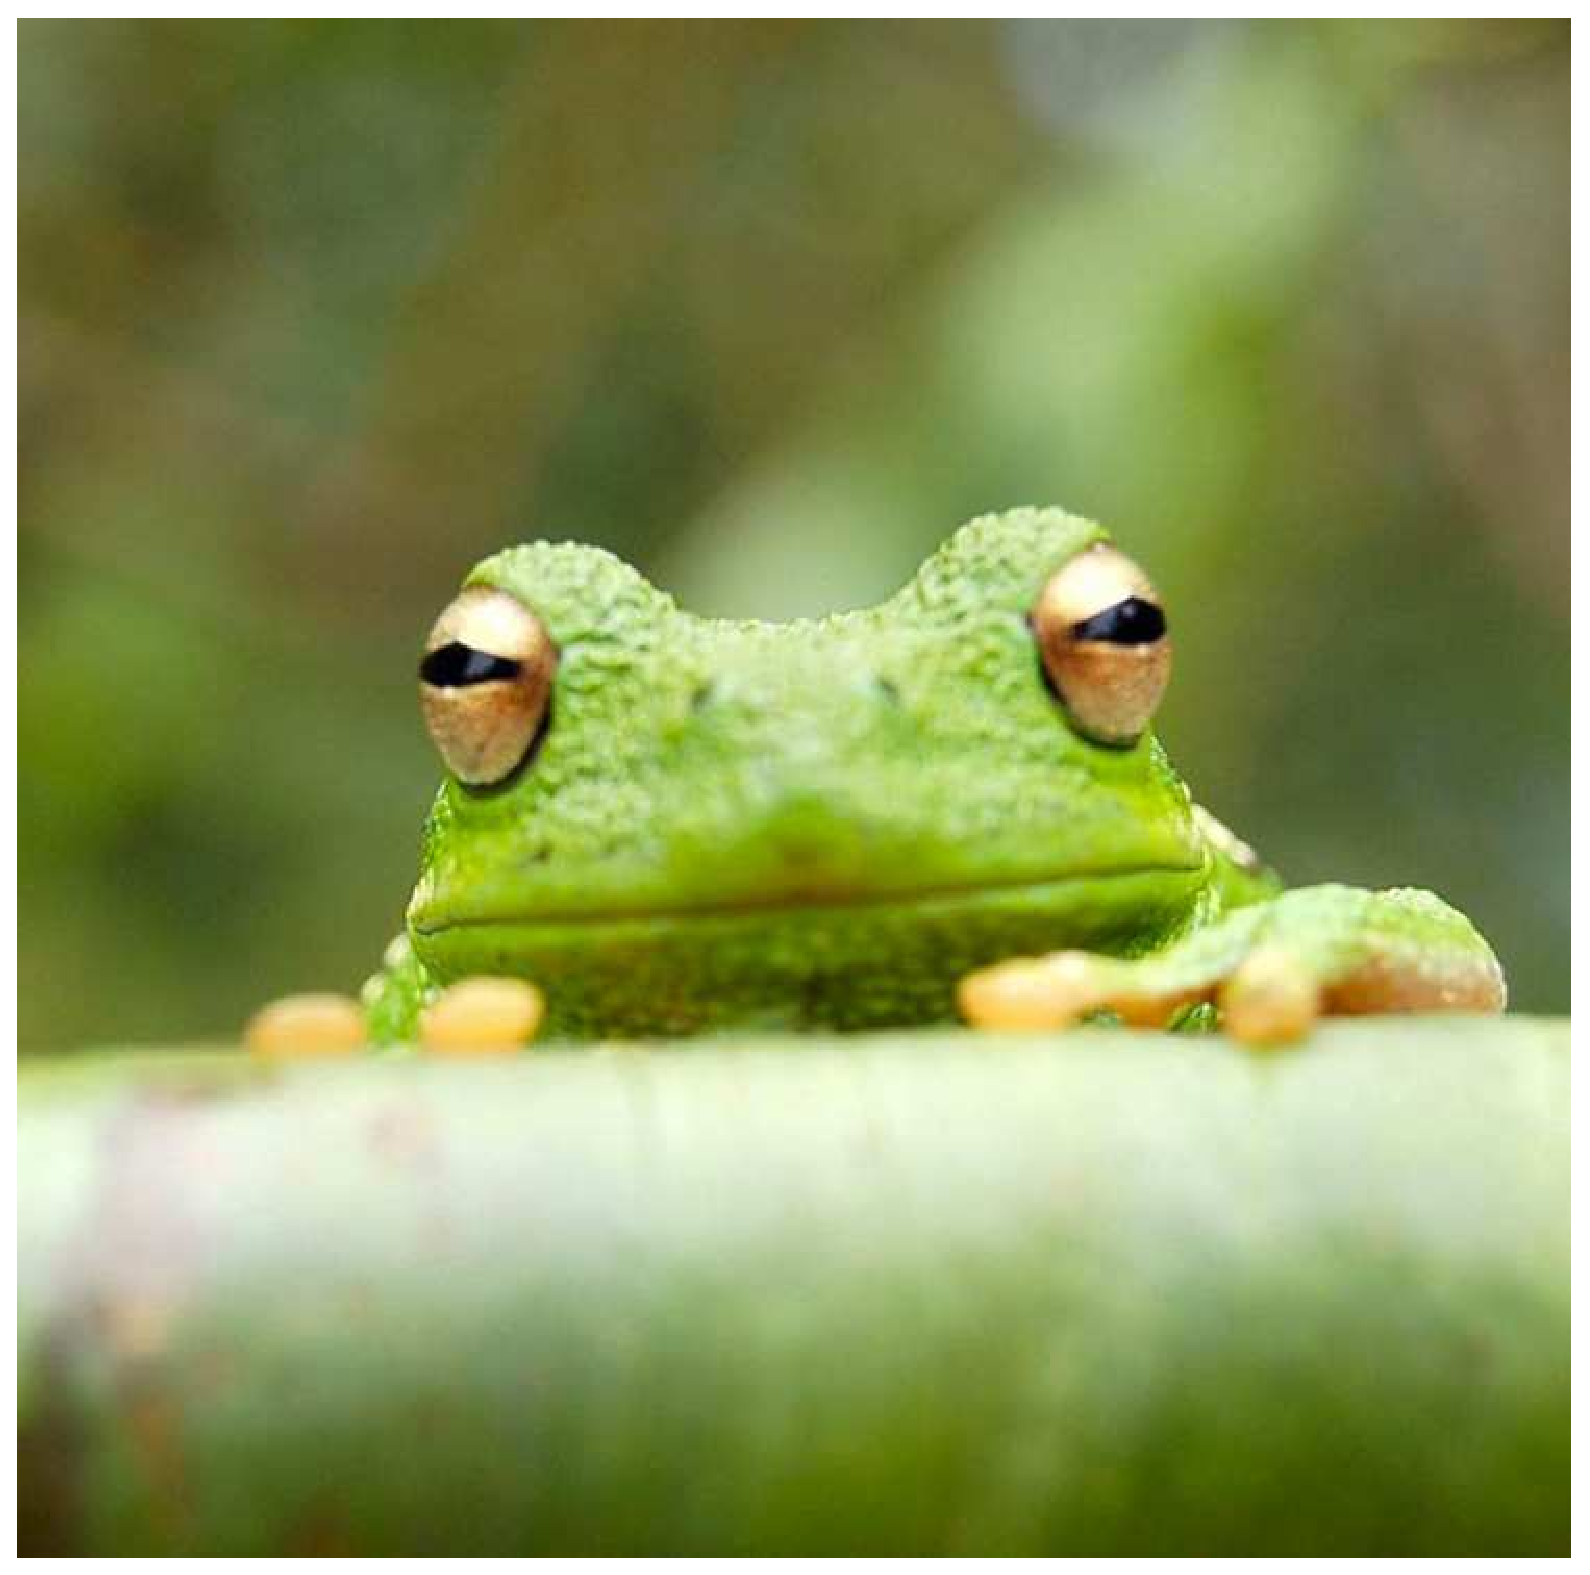
\includegraphics[width=.8\linewidth]{frog}
\caption{Placeholder image of a frog with a long example caption to show justification setting.}
\label{fig:frog}
\end{figure}


\begin{SCfigure*}[\sidecaptionrelwidth][t]
\centering
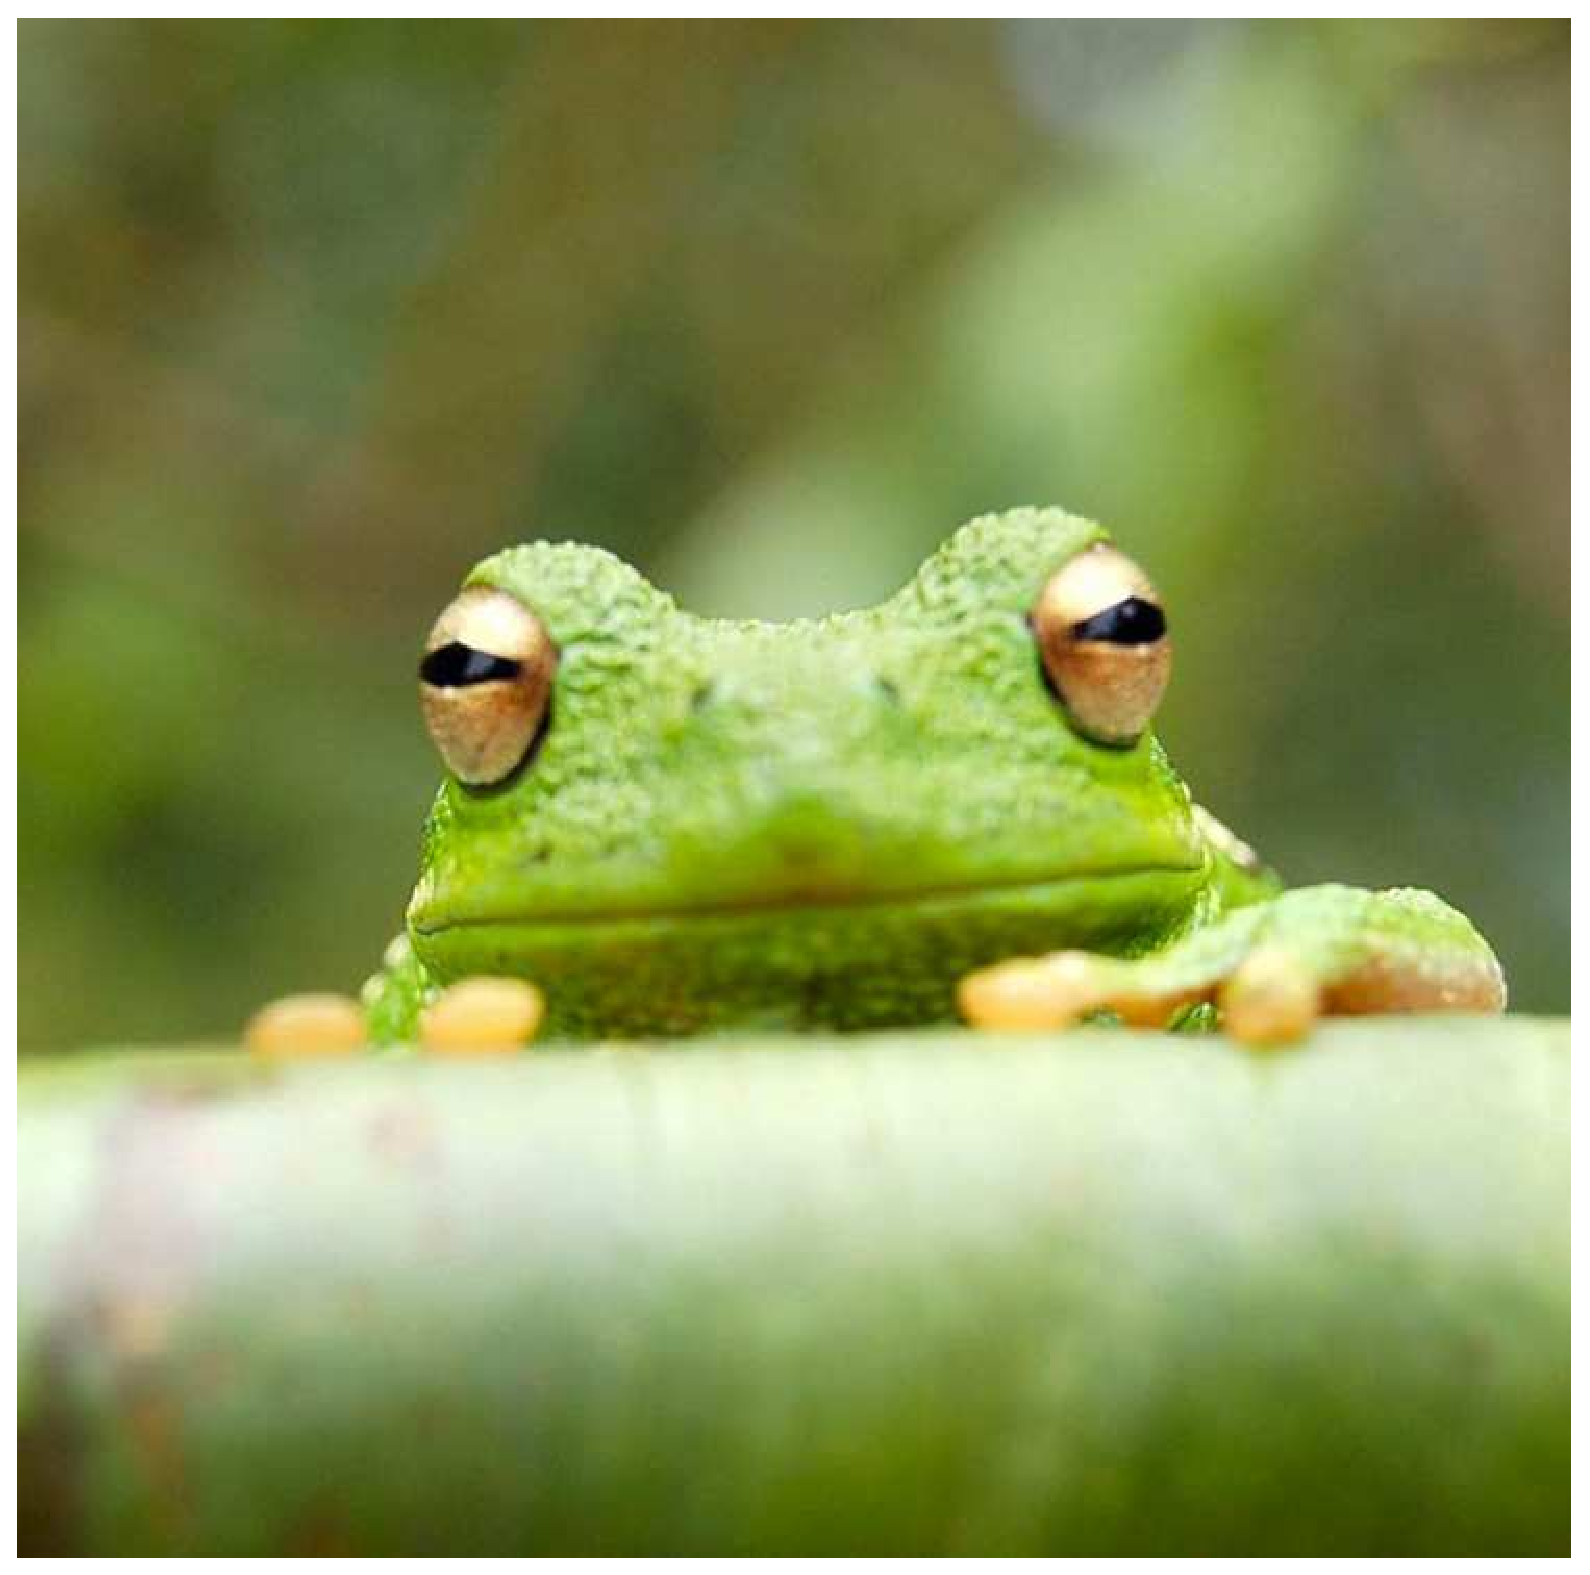
\includegraphics[width=11.4cm,height=11.4cm]{frog}
\caption{This caption would be placed at the side of the figure, rather than below it.}\label{fig:side}
\end{SCfigure*}

\subsection*{Digital Figures}

Only TIFF, EPS, and high-resolution PDF for Mac or PC are allowed for figures that will appear in the main text, and images must be final size. Authors may submit U3D or PRC files for 3D images; these must be accompanied by 2D representations in TIFF, EPS, or high-resolution PDF format.  Color images must be in RGB (red, green, blue) mode. Include the font files for any text. 

Figures and Tables should be labelled and referenced in the standard way using the \verb|\label{}| and \verb|\ref{}| commands.

Figure \ref{fig:frog} shows an example of how to insert a column-wide figure. To insert a figure wider than one column, please use the \verb|\begin{figure*}...\end{figure*}| environment. Figures wider than one column should be sized to 11.4 cm or 17.8 cm wide. Use \verb|\begin{SCfigure*}...\end{SCfigure*}| for a wide figure with side captions.

\subsection*{Tables}
In addition to including your tables within this manuscript file, PNAS requires that each table be uploaded to the submission separately as a “Table” file.  Please ensure that each table .tex file contains a preamble, the \verb|\begin{document}| command, and the \verb|\end{document}| command. This is necessary so that the submission system can convert each file to PDF.

\subsection*{Single column equations}

Authors may use 1- or 2-column equations in their article, according to their preference.

To allow an equation to span both columns, use the \verb|\begin{figure*}...\end{figure*}| environment mentioned above for figures.

Note that the use of the \verb|widetext| environment for equations is not recommended, and should not be used. 

\begin{figure*}[bt!]
\begin{align*}
(x+y)^3&=(x+y)(x+y)^2\\
       &=(x+y)(x^2+2xy+y^2) \numberthis \label{eqn:example} \\
       &=x^3+3x^2y+3xy^3+x^3. 
\end{align*}
\end{figure*}


\begin{table}%[tbhp]
\centering
\caption{Comparison of the fitted potential energy surfaces and ab initio benchmark electronic energy calculations}
\begin{tabular}{lrrr}
Species & CBS & CV & G3 \\
\midrule
1. Acetaldehyde & 0.0 & 0.0 & 0.0 \\
2. Vinyl alcohol & 9.1 & 9.6 & 13.5 \\
3. Hydroxyethylidene & 50.8 & 51.2 & 54.0\\
\bottomrule
\end{tabular}

\addtabletext{nomenclature for the TSs refers to the numbered species in the table.}
\end{table}

\subsection*{Supporting Information (SI)}

Authors should submit SI as a single separate PDF file, combining all text, figures, tables, movie legends, and SI references.  PNAS will publish SI uncomposed, as the authors have provided it.  Additional details can be found here: \href{http://www.pnas.org/page/authors/journal-policies}{policy on SI}.  For SI formatting instructions click \href{https://www.pnascentral.org/cgi-bin/main.plex?form_type=display_auth_si_instructions}{here}.  The PNAS Overleaf SI template can be found \href{https://www.overleaf.com/latex/templates/pnas-template-for-supplementary-information/wqfsfqwyjtsd}{here}.  Refer to the SI Appendix in the manuscript at an appropriate point in the text. Number supporting figures and tables starting with S1, S2, etc.

Authors who place detailed materials and methods in an SI Appendix must provide sufficient detail in the main text methods to enable a reader to follow the logic of the procedures and results and also must reference the SI methods. If a paper is fundamentally a study of a new method or technique, then the methods must be described completely in the main text.

\subsubsection*{SI Datasets} 

Supply Excel (.xls), RTF, or PDF files. This file type will be published in raw format and will not be edited or composed.


\subsubsection*{SI Movies}

Supply Audio Video Interleave (avi), Quicktime (mov), Windows Media (wmv), animated GIF (gif), or MPEG files and submit a brief legend for each movie in a Word or RTF file. All movies should be submitted at the desired reproduction size and length. Movies should be no more than 10 MB in size.


\subsubsection*{3D Figures}

Supply a composable U3D or PRC file so that it may be edited and composed. Authors may submit a PDF file but please note it will be published in raw format and will not be edited or composed.


\matmethods{Please describe your materials and methods here. This can be more than one paragraph, and may contain subsections and equations as required. Authors should include a statement in the methods section describing how readers will be able to access the data in the paper. 

\subsection*{Subsection for Method}
Example text for subsection.
}

\showmatmethods{} % Display the Materials and Methods section

\acknow{This research was supported by National Science Foundation Division of Environmental Biology awards 2208857 and 2225027. 
We thank the organizations and institutions who hosted us at their field station facilities, including The Nature Conservancy, Sam Houston State University, University of Texas, Texas A\&M University, Texas Tech University, Lake Lewisville Environmental Learning Area, Wichita State University, and Pittsburgh State University. }

\showacknow{} % Display the acknowledgments section

% Bibliography
\bibliography{Forecasting}

\end{document}